\documentclass[12pt,a4paper,utf8x]{report}
\usepackage [frenchb]{babel}
					
% Pour pouvoir utiliser 
\usepackage{graphicx}
%\usepackage[utf8x]{inputenc}

					
\usepackage{url} % Pour avoir de belles url
\usepackage {geometry}
\usepackage {setspace}
					
% Pour mettre du code source
\usepackage{listings}
\usepackage{color}
\usepackage{verbatim}
\usepackage{fancyvrb}

%% couleur java %%
\definecolor{javared}{rgb}{0.6,0,0} % for strings
\definecolor{javagreen}{rgb}{0.25,0.5,0.35} % comments
\definecolor{javapurple}{rgb}{0.5,0,0.35} % keywords
\definecolor{javadocblue}{rgb}{0.25,0.35,0.75} % javadoc

\lstset{
	language=Java,
	basicstyle=\footnotesize,
	numbers=left,
	numberstyle=\normalsize,
	breaklines=true,  
	numbersep=5pt,
	stepnumber=5,
	firstnumber=1,
 	numberfirstline=false,
	frame=single, 
	tabsize=2,
	keywordstyle=\color{javapurple}\bfseries,
	stringstyle=\color{javared},
	commentstyle=\color{javagreen},
	morecomment=[s][\color{javadocblue}]{/**}{*/},
}

\fvset{
	frame=single,
	fontsize==\footnotesize , 
	numbers=left,
}
%MODIF TITLE BY KEVIN
\title{Rapport}
\begin{document}
\maketitle
\clearpage

%FIN MODIF
\tableofcontents
\clearpage

% Pour avoir un interligne de 1,5
\begin{onehalfspace}
\chapter*{Introduction}
\addcontentsline{toc}{chapter}{Introduction}

\paragraph{}
Afin de valider les compétences acquises concernant la création d'application sur terminaux mobiles, les étudiants par groupe de quatre ont chacun reçu
un projet Android.

\paragraph{}
Notre sujet consiste à créer un \textbf{GPS piéton}. Ce GPS offrira plusieurs possibilités, deux principales
seront de retrouver des points d'intérêts, que nous appelleront par la suite \textbf{POI}, sur une carte ou à l'aide de la
réalité augmentée. Nous avons décidé d'utiliser Google API pour notre application. Ce choix est dû principalement au fait que certains 
membres du groupe ont déjà une premiere expérience sur ces API. 

\paragraph{}
Trois grandes idées de travails sont ressorties la récupérations de POI via le service Google, la réalité augmentée en utilisant la caméra, 
et le travail de calcul d'itinéraire sur la Map.

La première partie consiste à créér une classe permettant la communication entre notre application et la base de donnée à Google. La seconde utilise la
caméra afin d'afficher les POI sur l'écran, et la dernière partie utilise les informations reçues pour les afficher de manière classique sur une carte.

\clearpage
\chapter{Répartition du travail et travail réalisé}
\paragraph{}
Nous avions répartit les taches dès le debut du projet : Kevin souhaitait implémenter la réalité augmentée, Christophe et Benoit se sont chargés de comprendre comment nous pouvions interroger un service web pour récupérer des informations Géolocalisées.
Nicolas avait choisis de se charger de la partie d'affichage de la carte, et de la gestion de l'itinéraire étant donné qu'il connaissait déjà ces problèmes de part un sujet de stage similaire qu'il a réalisé par le passé.

\begin{center}
%	\includegraphics[width=140mm]{images/diag.png}
\end{center}

\paragraph{}
Nous aurions voulu présenter une application plus complète, qui permette a la fois de consulter un résultat via la réalité augmentée ainsi que via la carte. Mais la carte n'a pas été implémentée de manière fonctionnelle.

\clearpage
\chapter{Récupération des informations de lieu}
\paragraph{}
Un des points important du sujet est la récupérations de points d'intérêts. Pour ce faire il nous fallait utiliser des services en ligne, mais quel service ?

\section*{Quelle API choisir ?}
\paragraph{} 
Dans un premier temps, nous avions opter pour une solution se dissociant de Google, OpenStreetMap. Après quelques recherches infructueuses de librairies ou d'explications claires, l'équipe décida de migrer vers une API déjà connu de certains membres, \textbf{Google API}.
\paragraph{}
OpenStreetMap est assez peu documenté sur le web : la page Wikipedia ne permet pas de savoir comment peuvent etre interrogées les données d'une carte. Nous avons compris que les données sont enregistrées en XML, avec un format spécifique, mais cette structure n'est pas définie clairement. Cela signifie que si nous voulions charger des résultats récupérés depuis OpenStreetMap, il nous aurait fallu parser nous même le Xml et implémenter des classes contenant les résultats.
Par ailleurs, il n'existe que très peu de tutoriaux détaillés permettant d'implémenter des fonctionnalités grâce a OpenStreetMap.
Etant donné que cela représentait une quantité de travail importante sans pour autant nous offrir plus de possibilités pour l'application, nous avons choisis après quelques semaines d'utiliser les librairies Google. Notre envie de découvrir OpenStreetMap nous a au final fais perdre du temps que nous aurions pu passer à implémenter l'application.
En l'occurence, l'API Google Place définit des dizaines de types de batiments, et il existe des services web que l'on peut interroger via des requetes Web, avec les paramètres de recherche dans l'URL.

\section*{Google Place}
\paragraph{}
Parmi les nombreuses fonctionnalités que propose le géant de l'internet, une en particulière a retenu notre attention, une librairie permettant de récupérer les informations des lieux, Google Place API. Cette dernier nous permet de consulter, comme sur les applications maps du même groupe, les caractéristiques des lieux enregistrés dans leur base de données.

\section*{Comment cela fonctionne-t-il ?}
\paragraph{}
Le principe de l'API de d'envoyer des requêtes http au serveur afin de recevoir les points d'intérêts demandés.

\subsection*{les différents requêtes}
\paragraph{}
Nous utilisons quatres types de requêtes pour ce service.

\subsubsection*{Les recherches de proximité}
\paragraph{}
La recherche de proximité permet la récupération de tous points d'intérêts (cinéma,banque ...) dans un rayon maximal de 50km autour de la position de l'utilisateur.

\subsubsection*{Les recherches par texte}
\paragraph{}
Cette partie permet a l'utilisateur de recherche un lieu a partir du texte entrée.
Par exemple, s'il saisit « \textbf{Pizza Orléans} », il retournera les lieux en rapport avec pizza et Orléans.

\subsubsection*{La demande de détails}
\paragraph{}
Cette requête est très utile car par défaut, nous récupérons un lieu vraiment basique (nom, adresse, etc). Elle nous permet de compléter le lieu avec des informations complémentaires qui vont du site internet jusqu'aux commentaires ajouté par les utilisateurs de Google en passant par les horaires d'ouverture.
Dans notre cas nous utilisons que des informations simple comme le site web.

\subsubsection*{La récupération de photo}
\paragraph{}
Cette derniere permet de récupérer via une référence, une url poitant vers la photo d'un lieu.

\subsection*{Les résultats obtenus}
\paragraph{}
L'usage de cette librairie nous renvoi les données au format JSON. Afin de les rendre utilisable, le résultat est directement transformer en classe par le biais d'un parseur. Celui-ci est créer lors de la génération du transporteur HTTP dans la classe FouilleDonnee.

\subsection*{Le code}
\paragraph{}
Comme tous service de Google l'exige, il a fallu enregistrer le projet afin d'obtenir une clé nous autorisant à se connecter aux serveurs. La norme Android spécifie d'utiliser cette classe dans une classe asynchrone.
\clearpage
\subsubsection*{Les requêtes}
\paragraph{}
Voici une des requêtes concernant la récupération de point d'intérêts
\\
\end{onehalfspace}
\begin{lstlisting}
	public ListeLieu getLieuProximiteParType(double lat,double lng,ArrayList<String> types,int distance) {
		try {

			HttpRequestFactory httpRequestFactory = createRequestFactory(HTTP_TRANSPORT);
			HttpRequest request = httpRequestFactory
					.buildGetRequest(new GenericUrl(PLACES_SEARCH_URL));


			request.getUrl().put("location", lat + "," + lng);
			request.getUrl().put("radius", distance); // in meters

			if(types != null && types.size()>0) {
				types=FrancaisToApi(types);
				request.getUrl().put("types", typesFormatUrl(types));
			}
		
			completePlaceQuery(request.getUrl());
			Log.d("url",request.getUrl().toString());
			ListeLieu list = request.execute().parseAs(ListeLieu.class);
			return list;

		} catch (HttpResponseException e) {
            Log.e("Error:", e.getMessage());
        } catch (IOException e) {
			e.printStackTrace();
		//} catch (InterruptedException e) {
			//e.printStackTrace();
        } 
		return null;
	}
\end{lstlisting}
\begin{onehalfspace}
\subsubsection*{Lieu}
\paragraph{}
Sur chaque membre de la classe nous ajoutons l'annotation @Key afin que le parseur remplisse chaque champs de la classe avec le code JSON. Afin de filtrer les informations dont nous n'avons pas besoin, comme les commentaires d'utilisateurs de Google, il suffit de ne pas mettre de champs correspondant.
\\
\end{onehalfspace}
\begin{lstlisting}
//Il faut que cette classe soit serializable pour appliquer le writeObject() dessus
public class Lieu implements Serializable{

	private static final long serialVersionUID = 1L;

	public Lieu(){
	}
	/**
	 * L utilisateur veut enregistrer sa position actuelle comme favoris
	 * Il saisis certains champs seulement, et l'id n'est pas connu
	 * @param name
	 * @param reference
	 * @param icon
	 * @param vicinity
	 * @param geometry
	 * @param formatted_address
	 */
	public Lieu(String name, List<String> types , String reference, String icon, String vicinity, Geometry geometry, String formatted_address,String phoneNumer,String website){
		id="";
		this.types = types;
		this.name=name;
		this.reference=reference;
		this.icon=icon;
		this.vicinity=vicinity;
		this.geometry=geometry;
		this.formatted_address=formatted_address;
		this.formatted_phone_number = phoneNumer;
		this.website = website;
	}

	@Key	
	public String id;
	@Key
	public String name;
	@Key
	public String reference;
	@Key
	public String icon;
	@Key
	public String vicinity;
	@Key
	public Geometry geometry;
	@Key
	public String formatted_address;
	@Key 
	public List<Photo> photos;
	@Key
	public List<String> types;
	/** DETAILS */
	@Key
	public String formatted_phone_number;
	@Key
	public String website;
	@Override
	public String toString() {
		return id+" "+name+" "+icon;
	}

	public static class Geometry implements Serializable
	{
		private static final long serialVersionUID = -1846546423355113268L;
		@Key
		public MyLocation location;
		
		public Geometry(){	
		}
		
		public Geometry(MyLocation location){
			this.location=location;
		}
	}

	public static class MyLocation implements Serializable
	{
		private static final long serialVersionUID = -745398283024148157L;
		
		@Key
		public double lat;
		@Key
		public double lng;
		
		public MyLocation(){	
		}
		
		public MyLocation(double lat, double lng){
			this.lat=lat;
			this.lng=lng;
		}
	}

	public double getLatitude() {
		return geometry.location.lat;
	}

	public double getLongitude() {
		return geometry.location.lng;
	}

	@Override
	public boolean equals(Object o) {
		Lieu l = (Lieu)o;
		return this.name==l.getNom();
	}
}
\end{lstlisting}
\begin{onehalfspace}
\subsubsection*{ListeLieu}
\paragraph{}
Cette classe correspondant à la racine du JSON, le status nous permet de savoir comment la requête s'est déroulée, \textbf{next\_page\_token} permet d'avoir acccès au 20 résultats suivants dans une limite de 60 par requêtes et la liste de Lieu contient tous les lieux que la requête a demandée.
\\
\end{onehalfspace}
\begin{lstlisting}
public class ListeLieu implements Serializable {
 
    private static final long serialVersionUID = -1467727864221797449L;

    @Key
    public String status;
	
    @Key
    public String next_page_token;
 
    @Key
    public List<Lieu> results;
 
}
\end{lstlisting}
\begin{onehalfspace}
\subsubsection*{PlaceDetails}
\paragraph{}
Cette classe, comme ListeLieu correspondant a la racine du retour de notre requête concernant la demande de détails sur un lieu, elle contient un lieu et le status de la requête.


\paragraph{}
Ces classes forment la liaison entre notre application et les serveurs de Google. Mais existe-t-il d'autres hébergeurs pour ce type de services ?

\section*{Et pourquoi pas quitter Google ?}
\paragraph{}
Les plateformes à Google étant gratuites et mondialement connues, ils doivent donc limiter les usages de leurs services, alors autres que récupérer toutes vos informations, ce dernier bride le nombre de requêtes pour chaque services, dans notre cas nous atteignons la barre de 1000 requêtes par jour, ridicule. 
\paragraph{}
Il nous est possible de dépasser cette limitation mais tout en restant « gratuit » par l'enregistrement d'une carte bancaire, impensable pour nous. De ce faite, vous pensions à nouveau migrer vers un autre hébergeur pour ce service.
\paragraph{}
En effet, il existe \emph{FourSquare} ou \emph{Yahoo GeoPlanet}, qui propose les mêmes fonctionnalités. Si l'envie en prenait aux développeurs de migrer vers ces plateformes, il ne suffirait que de modifier les fonctions associés aux requêtes afin de se désenchaîner de ce géant.

\clearpage
\chapter{Gestion de la carte}

\section{La carte}
On utilise la carte de l'api google maps. L'ativité qui gère la carte devra utiliser la classe MapActivity au lieu d'Activity.\\

L'utilisateur a besoin de pouvoir zoommer sur la carte, pour cela on utilise la fonction  mapView.setBuiltInZoomControls(true) qui nous permet le zoom et aussi cette fonction permet au téléphone qui n'on pas de multitouch de pour zoomer grâce au boutonnqui s'affiche suite au clic sur la carte. \\

Ensuite nous avons besoin d'un controleur qui va nous permettre de façon interne de pourvoir effectuer un zoom ou de placer la carte sur un point précis. Par exemple au premier affichage de la carte, on va centrer la carte sur notre possition. \\

L'objet MyLocationOverlay va nous permetre de connaitre la position de l'utilisateur et aussi d'ajouter un overlay à la carte qui sera la position de l'utilisateur. \\

\section{Gestion des POI}

Un point d'intéret sera caractérisé par un OverlayItem qui sera afficher sur la carte. pour stocker nos points d'intérets, on a créé la classe ListItemizedOverlay qui contient une liste de tout les POI. Cette classe contient un Drawable qui sera l'icone associé à notre point. \\

L'utilisateur pour cliquer sur chacun de ces points. ainsi il accedera aux informations de ce point, donc l'adresse, numéro de téléphone, ... Ensuite depuis cette fenêtre il pourra décider de créer un itinéraire vers ce point en mode statique, il y aura juste le tracé de l'itinéraire sur la carte. Sinon l'utilisateur pourra choisir d'utiliser la navigation. \\

 

\clearpage				
\chapter{Réalité Augmentée}

  \section*{Vue Personnalisée}
  
    \paragraph{}
    Pour pouvoir afficher les icônes sur la caméra, il fallait dans un premier temps pourvoir gérer l'ouverture et la fermeture de celle-çi. Pour cela 
    nous avons dû avoir recours à une vue personnalisée. La vue personnalisée récupère les paramètres de la caméra du mobile, elle créée une surface que
    l'on va pourvoir utiliser dans nos layouts en mettant le chemin de notre classe.
    
    \end{onehalfspace}
    \begin{lstlisting}
<com.example.eyeway.realiteAugmente.CustomCameraView
        android:id="@+id/camera"
        android:layout_width="wrap_content"
        android:layout_height="wrap_content" />
    \end{lstlisting}
     \begin{onehalfspace}
  \section*{Positionner les points d'intérêt}
    
    \paragraph{}
    
    Le second travail est l'un des plus important de la partie réalité augmentée, il s'agit du positionement des points d'intérêt sur la caméra. Nous devons 
    pour cela récupèrer la position actuelle de l'utilisateur et la position du point d'intérêt. Nous faisons ensuite un calcul d'angle en récupèrant 
    l'angle entre nous et le nord ainsi que celui entre nous et le point d'intérêt. Ceci va nous permettre de savoir en fonction de l'orientation du téléphone
    , les points d'intérêt se trouvant dans la direction regardée par l'utilisateur.
    
    \paragraph{}
    Pour récupèrer notre position actuelle nous avons accès à deux ressources, le GPS  et le réseau du téléphone. Chacune de ces ressources comportent
    ses inconvénients et ses avantages. Le GPS a l'avantage d'être précis mais il a pour inconvénient d'être lent à se mettre en route dans certains cas
    d'utilisations, par exemple dans un bâtiment. Le réseau lui est plûtot rapide mais il comporte une marge d'erreur vraiment importante. 
    
    \paragraph{}
    Nous avertissons donc l'utilisateur lorsque le GPS n'est pas activé, en lui indiquant que sans l'utilisation de celui-çi l'application sera moins précise. Nous 
    avons donc absolument besoin de l'un ou de l'autre, c'est pourquoi nous bloquons l'utilisation de la géocalisation si l'itinérance de données n'est
    pas activée ou au moins une des deux ressources n'est pas activée.
    
    
    \paragraph{}
    L'étape suivante pour le positionement d'un point d'intérêt était de savoir en fonction de l'angle où le postionner sur l'écran. Pour cela nous 
    avons utilisé l'attribut margin pour placer l'imageView sur l'écran, nous récupèrons ainsi la hauteur, la largeur de l'écran, les valeurs renvoyées
    par l'accélérometre du téléphone et nous utilisons un calcul trouvé sur internet qui permet à partir de ces valeurs de connaître la position du point d'intérêt
    sur l'écran.
    
    \paragraph{}
    Chaque point d'intérêt aura une icône en relation avec son type de batîments et un label qui correspondra à la distance entre la position actuelle 
    de l'utilisateur. Nous devons donc pour chaque point d'intérêt recalculer le label lorsque la position de l'utilisateur change. Nous avons mis une
    icône par défaut si le type de batîment n'est pas connu.
    
    
    \section*{Création d'un nouveau point d'intérêt}

    \paragraph{}
    L'utilisateur peut à tout moment vouloir créer un nouveau point d'intérêt s'il le souhaite. Pour cela il devra appuyé quelques secondes sur l'écran,
    nous offrons la possibilité à l'utilisateur de renseigner certains champs : le nom, une description, l'adresse, le numéro de téléphone et le site 
    web de son nouveau point.
    
    \paragraph{}
    Nous pré-remplissons le champ adresse à l'aide de la classe GeoCoder qui permet de retourner en fonction d'une longitude
    et d'une lattitude l'adresse correspondante. L'utilisateur doit ensuite appuyé sur le bouton sauvegarder, ceci aura comme action de sauvegarder le 
    nouveau point comme favoris et de l'ajouter directement à l'écran. L'utilisateur pourra ensuite retrouver son nouveau point à chaque utilisation 
    de l'application dans le menu de gestion de favoris.
    
    \begin{center}
	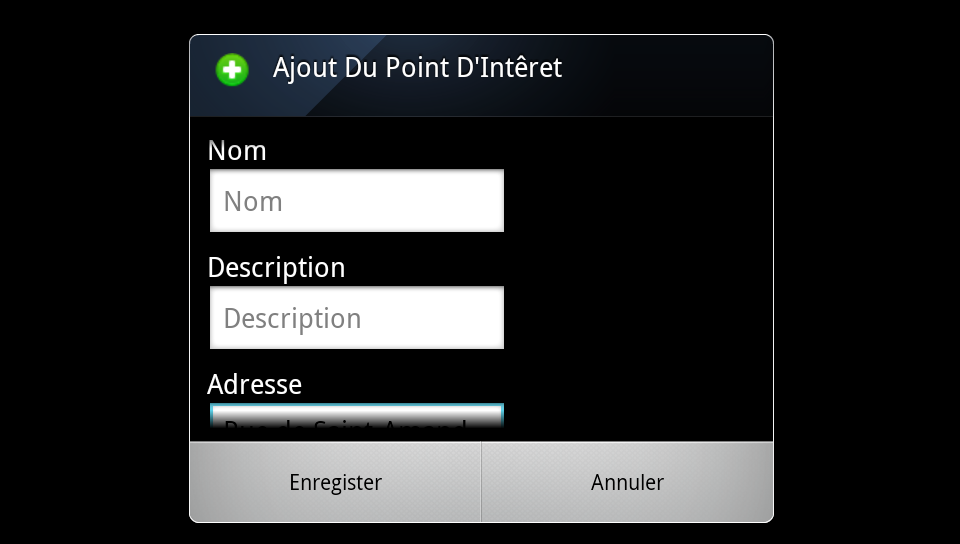
\includegraphics[width=140mm]{images/ajout_poi.png}
    \end{center}

      
    \section*{Détails d'un point d'intêret}
    
    \paragraph{}
    Pour avoir accès au détails d'un point d'intérêt, nous avons fait en sorte que les images soit cliquables. Donc lorsque l'utilisateur voudra le
    détails d'un certain point il devra juste cliquer sur l'icône en question. Lorsque le clic est effectué nous utilisons la requête de détails qui 
    va récupèrer le lieu complété avec les informations manquantes.
    
    \paragraph{}
    Une fois la requête executée nous affichons une boite de dialogue comportant tout les champs renseignés dans lieu. Et nous offrons aussi la possibilité
    à l'utilisateur de sauvegarder le lieu en question et de basculer vers la vue map pour calculer un itinéraire. La partie Map n'étant pas fonctionnelle
    nous avons pas eu la possibilité de l'utiliser.
    
    \begin{center}
	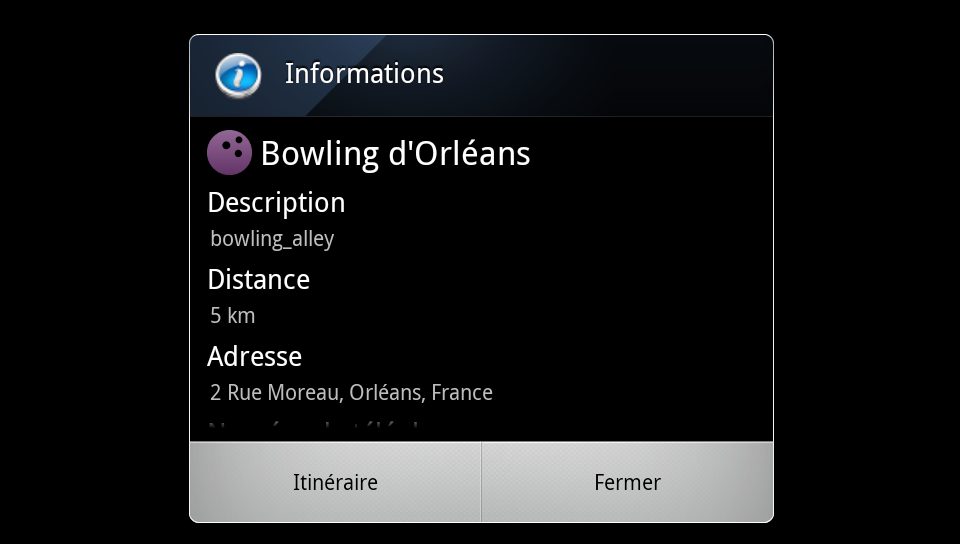
\includegraphics[width=140mm]{images/detail_poi.png}
    \end{center}
    
    \section*{Amélioration possible}
    
    \paragraph{}
    Pour la réalité augmentée nous aurions aimé pouvoir implémenter un systéme de guidage vers un point d'intérêt sélectionné par l'utilisateur. Pour 
    cela nous avions penser à utiliser une fléche qui dirigerais l'utilisateur vers sa destination.
\clearpage
\chapter{Interface}

\section*{Implémentation des layouts}
\paragraph{}
Les layouts sont la mise en forme des différentes pages de l'application. Android propose des attributs prédéfinis pour paramétrer l'affichage des composants (chaque composant Android est une View). Nous avons été plus loin que les attributs prédéfinis en Android : Christophe souhaitait par exemple avoir des éléments avec des bords arrondis, des background en couleur dégradées, etc.
Pour cela, il a fallu utiliser les drawable, a définir dans une fichier Xml, puis a appliquer sur les View concernées : 

\begin{center}
	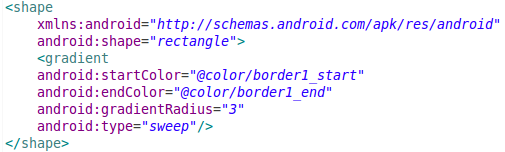
\includegraphics[width=140mm]{images/drawable.png}
	Drawable définissant les bords arrondis
\end{center}

\paragraph{}
Les différentes listes visibles dans l'application (par exemple la liste des fonctionnalités sur le menu principal) sont gérées par un fichier Xml qui défini la liste en elle même, et un fichier Xml qui définit un élément de cette liste. La encore il s'agit d'étendre ce qui est offert de base par android : les items d'une listview par défaut ne peuvent contenir qu'une String, alors que dans notre cas nous voulons afficher une icone et une String. Cela est rendu possible par l'heritage de la classe Adapter. Dans le cas d'une listview que l'on veut mettre a jour au cours de la vie de l'application, il faut implémenter la méthode notifyDataSetChanged() et l'appeler explicitement afin de rafraichir la ListView.

\begin{center}
	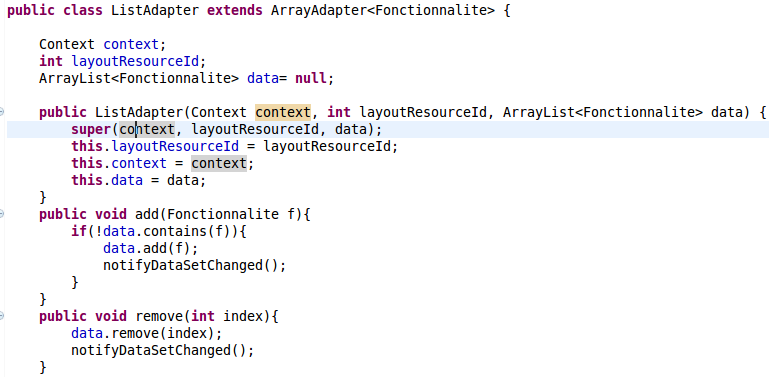
\includegraphics[width=140mm]{images/list_adapter.png}
	Adapter permettant la création d'un listview personnalisée
\end{center}

\paragraph{}
Lorsque nous avons testé l'application sur une tablette, nous nous sommes apercus que l'affichage du menu était trop petit sur une tablette, et lorsqu'il était correct sur tablette, les éléments étaient trop grand sur telephone. Nous avons gérer ces deux cas en détectant le périphérique sur lequel est lancé l'application et en appliquant un layout différent.

\begin{center}
	\fbox{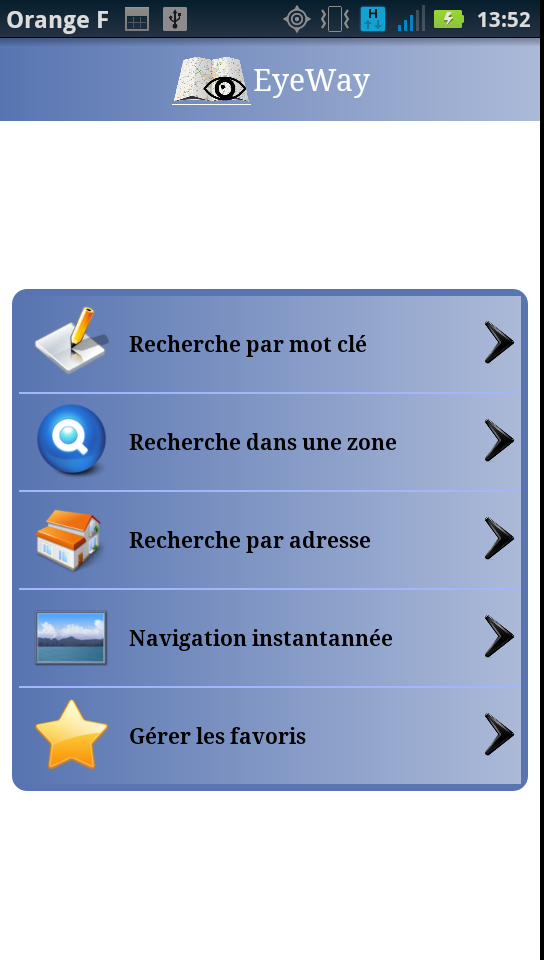
\includegraphics[width=60mm]{images/menu_principal.png}}
\end{center}

\begin{center}
	\fbox{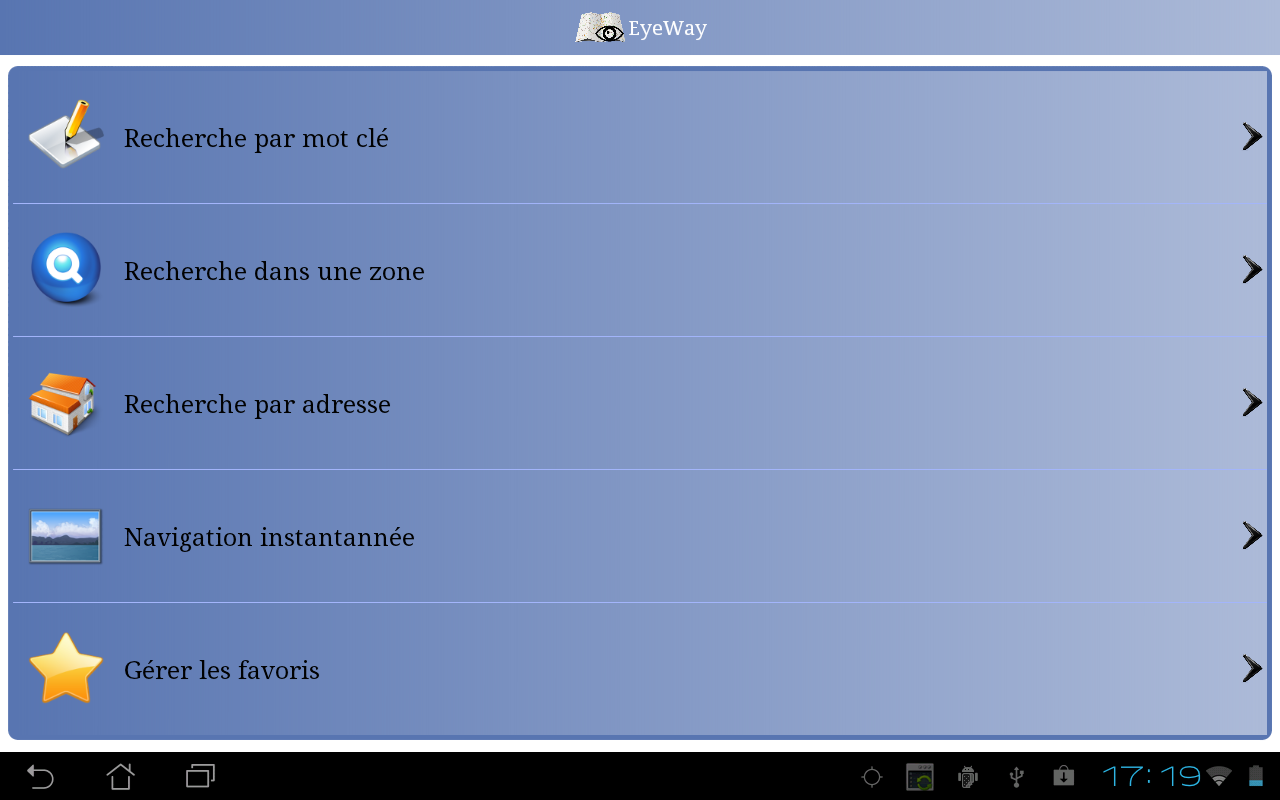
\includegraphics[width=140mm]{images/menu_tablette.png}}
\end{center}

\paragraph{}
Nous avons créer un bandeau contenant le nom et l'icône de l'application visible sur chaque page. Ce bandeau consiste en un fichier xml, chargé par les différents layout grâce à la directive include.
\section*{Gestion du swipe}
\paragraph{}
Nous avons implémenté le swipe sur différents formulaires afin de revenir sur le menu principal.

\section*{Gestion de l'orientation}
\paragraph{}
Lorsque l'orientation du terminal change, android fait un appel au onCreate() de l'application, ce qui a pour effet de perdre les saisies de l'utilisateur. C'est le cas dans la recherche par perimètre avec la liste des types extensible.
Nous avons géré le changement d'orientation en restaurant les types saisis par le passé.

\section*{AlertDialog customisée}
\paragraph{}
De base, Android ne permet de créer que des AlertDialog contenant un texte, et pour afficher un favoris ou bien un résultat de la recherche, nous avions besoin d'afficher le nom du lieu, l'adresse, la ville, le site web...
Nous avons utilisé des AlertDialog customisés, qui contiennent un layout définit la encore par un fichier Xml. 

\begin{center}
	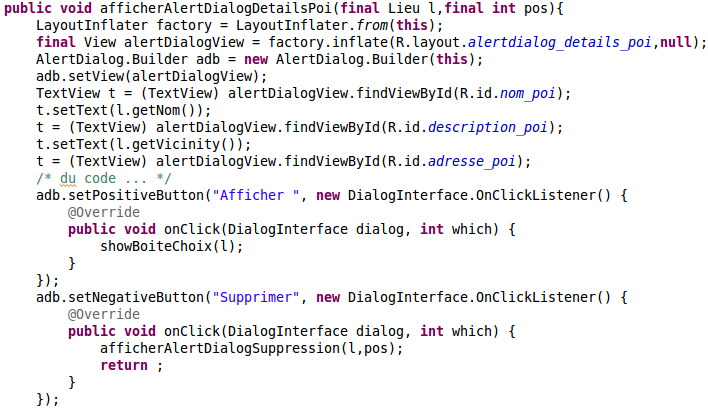
\includegraphics[width=140mm]{images/alertdialog.png}
	AlertDialog permettant de voir un favoris enregistré 
\end{center}
\paragraph{}
On a aussi construit une classe AlertDialogManager qui permet de contenir la définition des AlertDialog personnalisés de l'application, de manière a factoriser le code et a le rendre simple a utiliser.

\section*{Choix de l'affichage}
Pour chaque formulaire il est possible de consulter les résultats via la map ou la réalité augmentée par le biais d'une boite de dialogue.

\begin{center}
	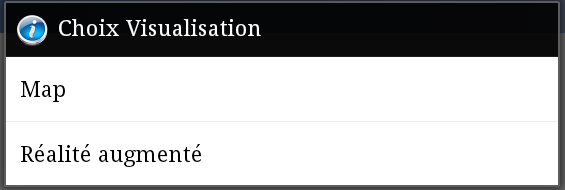
\includegraphics[width=140mm]{images/choix.png}
\end{center}


\section*{Affichage et sauvegarde des favoris}

\paragraph{}
Nous avons géré la sauvegarde d'un point d'intéret, de manière a ce que l'utilisateur puisse conserver les lieux qu'il a consulté. Pour cela, l'utilisateur peut rester appuyé sur l'ecran de réalité augmentée ou bien lorsqu'il consulte le détail d'un résultat.
\paragraph{}
L'affichage est confié a une listview extensible et rafraichie automatiquement (comme expliqué précédemment pour la listview des types pour la recherche par perimètre). 
\paragraph{}
La sauvegarde des favoris est faite avec des enregistrements dans l'internal storage Android.
Pour enregistrer un Lieu, il faut que cette classe soit serializable, puis il faut convertir l'objet concerné en tableau de bytes, et appeler la méthode write() :

\begin{center}
	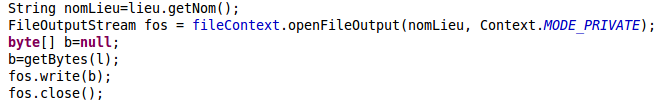
\includegraphics[width=140mm]{images/fichier.png}
\end{center}


\paragraph{}
Nous conservons dans l'application les favoris enregistrés, et il est possible de supprimer un favoris, ce qui va supprimer le fichier concerné dans l'internal storage.

\clearpage
%\input{conclusion}

\end{onehalfspace}
\end{document}
